\documentclass[handout,aspectratio=169]{beamer}
\usepackage{graphicx}
\usepackage{booktabs}
\usepackage{array}
\usepackage{listings}
\usepackage{xcolor}

\definecolor{codegreen}{rgb}{0,0.6,0}
\definecolor{codegray}{rgb}{0.5,0.5,0.5}
\definecolor{codepurple}{rgb}{0.58,0,0.82}
\definecolor{backcolour}{rgb}{0.95,0.95,0.92}

\lstset{
    backgroundcolor=\color{backcolour},
    commentstyle=\color{codegreen},
    keywordstyle=\color{magenta},
    numberstyle=\tiny\color{codegray},
    stringstyle=\color{codepurple},
    basicstyle=\ttfamily\scriptsize,
    breakatwhitespace=false,
    breaklines=true,
    captionpos=b,
    keepspaces=true,
    numbers=left,
    numbersep=5pt,
    showspaces=false,
    showstringspaces=false,
    showtabs=false,
    tabsize=2
}

\title{Re-processing Perturb-Seq datasets from FASTQ}
\subtitle{First Results for the Unified Pipeline}
\date{2026-05-07}
\author{Kirill Tsukanov \\ Senior Full Stack Developer \& Data Engineer \\ \texttt{ktsukanov@ebi.ac.uk}}
\institute{Perturbation Catalogue Fortnightly Meeting}

\setbeamertemplate{navigation symbols}{}
\setbeamertemplate{footline}{%
  \begin{beamercolorbox}[wd=\paperwidth,ht=2.5ex,dp=1.5ex,center]{}
    \hspace{15pt}\usebeamerfont{author in head/foot}Unified FASTQ Re-analysis Pipeline
    \hfill
    \usebeamerfont{date in head/foot}\insertframenumber{} / \inserttotalframenumber
    \hspace{15pt}
  \end{beamercolorbox}%
}

\begin{document}

\begin{frame}
    \titlepage
\end{frame}

\begin{frame}{Why re-process from FASTQ?}
    \begin{itemize}
        \item \textbf{Consistency:} scPerturb datasets are usually deposited as processed H5AD files, but they come from different pipelines, references, and filtering choices.
        \item \textbf{Comparable outputs:} Re-processing gives us a common count matrix layout, common metadata expectations, and a consistent way to attach guide counts.
        \item \textbf{Quality control:} Raw reads let us apply the same checks across studies instead of inheriting every author-specific decision.
        \item \textbf{Catalogue expectation:} Users expect harmonised data in the Perturbation Catalogue, not only links to heterogeneous processed files.
    \end{itemize}
\end{frame}

\begin{frame}{Why Kallisto + Bustools?}
    \begin{itemize}
        \item \textbf{Speed:} Kallisto + Bustools is much faster than Cell Ranger while giving very comparable expression quantification.
        \item \textbf{Resource fit:} We have adequate, but not unlimited, compute and storage. The pipeline must work within those limits.
        \item \textbf{Full catalogue scale:} We want to process all datasets we have, and be able to reprocess them if the pipeline improves.
        \item \textbf{Future-proofing:} New perturb-seq datasets are expected to be very large, so the pipeline needs to scale well rather than depend on throwing more hardware at each run.
    \end{itemize}
\end{frame}

\begin{frame}{Pipeline Architecture}
    \centering
    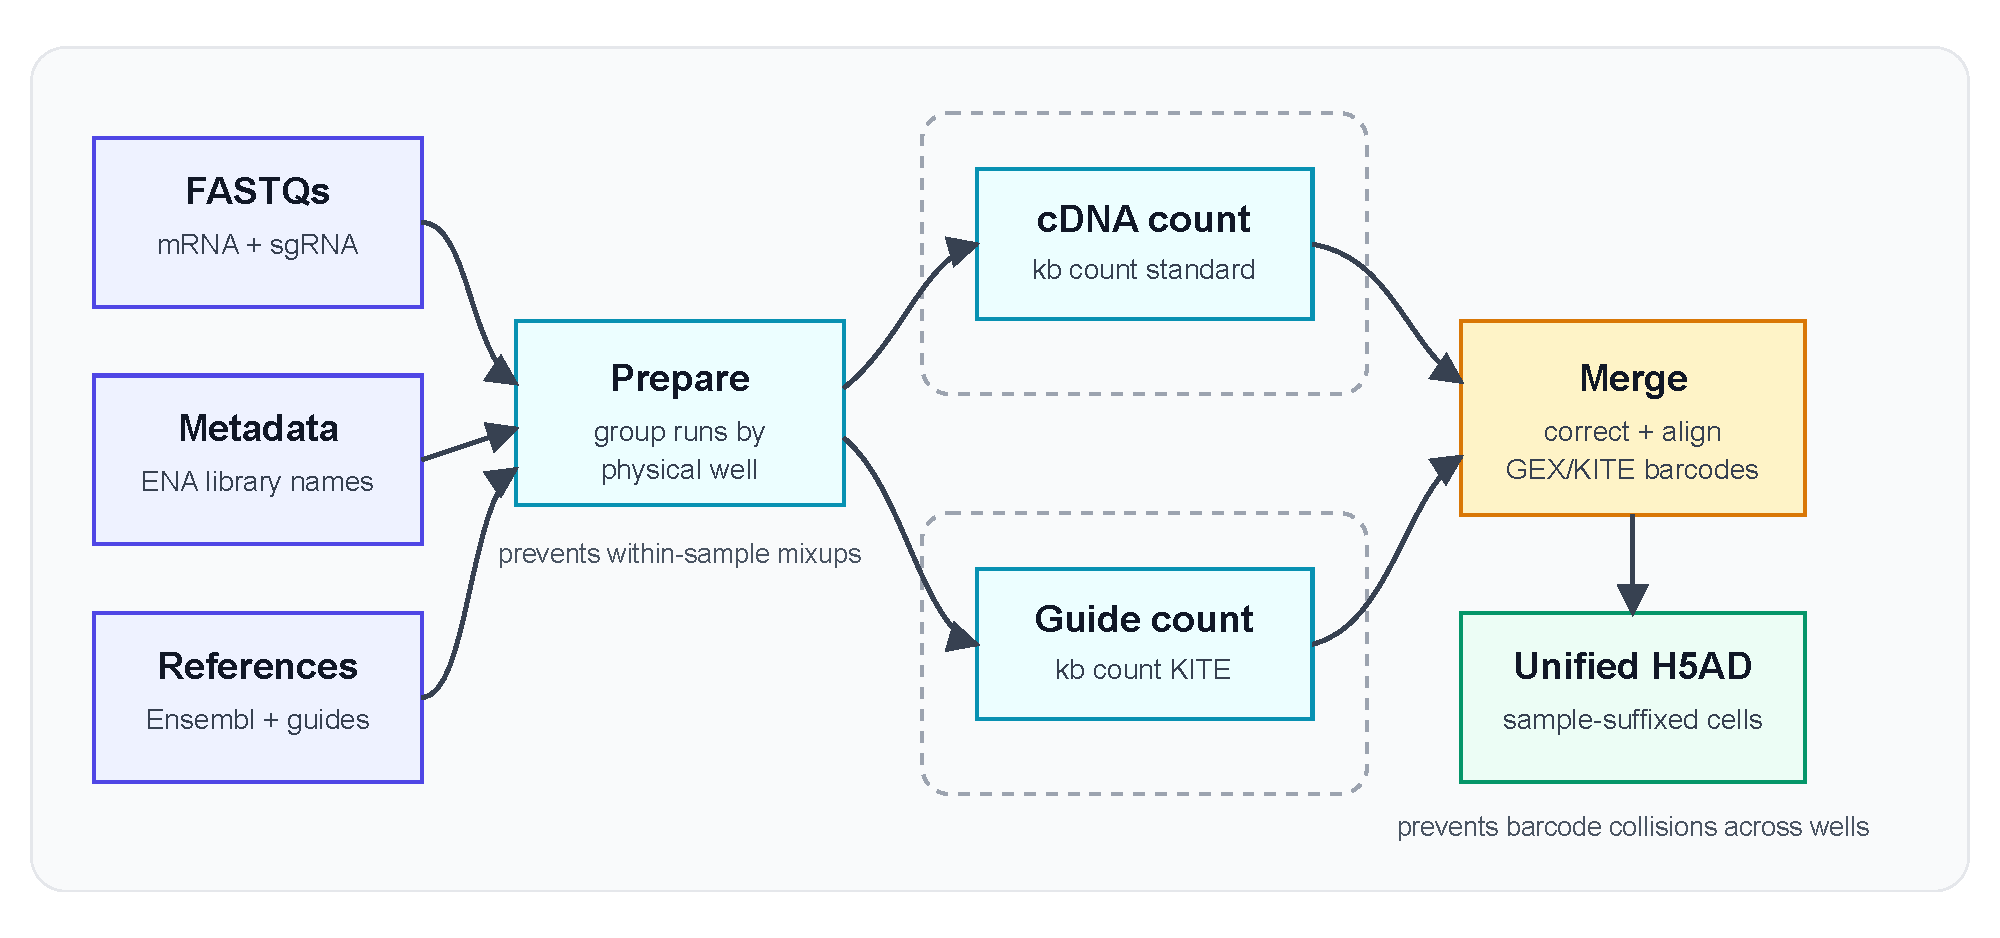
\includegraphics[width=0.98\linewidth,height=0.78\textheight,keepaspectratio]{pipeline_workflow.pdf}
\end{frame}

\begin{frame}{Development Issues Solved}
    \begin{itemize}
        \item \textbf{ENA FASTQs missing technical reads:} Historical ENA FASTQs for this dataset do not include the barcode/UMI reads. Current workaround: SRA download with technical reads included. We notified ENA; they are aware and plan to fix it, so future runs may use ENA directly.
        \item \textbf{Sample grouping:} SRRs and lanes must be grouped by physical well before counting. This is currently parsed from ENA library names; later versions may autodetect this.
        \item \textbf{Barcode collisions:} Final concatenation adds sample suffixes so identical 10x barcodes from different wells remain distinct.
        \item \textbf{GEX/KITE matching:} Guide barcodes are not exactly the same as expression barcodes in this dataset. The pipeline applies the required KITE barcode correction before alignment.
    \end{itemize}
\end{frame}

\begin{frame}[fragile]{Pipeline Execution}
\begin{lstlisting}[language=bash]
nextflow run main.nf \
  -profile slurm,singularity \
  --fastq_dir $HPS_PATH/perturb_seq_fastq/SAMN40972597 \
  --metadata_tsv $HPS_PATH/perturb_seq_fastq/SAMN40972597/ena_metadata.tsv \
  --outdir $HPS_PATH/perturb_seq_fastq/results \
  --chemistry 10xv3 \
  --transcriptome_fa $HPS_PATH/cache/reference/Homo_sapiens.GRCh38.dna.primary_assembly.fa.gz \
  --gtf $HPS_PATH/cache/reference/Homo_sapiens.GRCh38.111.gtf.gz \
  --features_tsv $HPS_PATH/perturb_seq_fastq/SAMN40972597/features.tsv
\end{lstlisting}
    \vspace{0.4em}
    \begin{itemize}
        \item The sample sheet is generated automatically from ENA metadata.
        \item mRNA and sgRNA workflows run in parallel per sample.
        \item Guide counts are merged from unfiltered KITE output, then aligned to filtered mRNA cells.
    \end{itemize}
\end{frame}

\begin{frame}{First Dataset: Nadig 2025 Jurkat}
    \begin{itemize}
        \item The unified FASTQ-to-H5AD pipeline now runs end-to-end on the EBI Slurm cluster.
        \item The first full dataset has been processed: Nadig 2025 Jurkat.
        \item The comparison was run against the author-provided H5AD.
        \item Analysis compares shared cells and shared genes after barcode and gene-name alignment.
        \item The main question: does the reprocessed dataset reasonably reproduce the expression and guide signals?
    \end{itemize}
\end{frame}

\begin{frame}{First Dataset: Scale and Runtime}
    \begin{columns}[T,onlytextwidth]
        \begin{column}{0.49\textwidth}
            \textbf{Input scale}
            \vspace{0.5em}
            \begin{itemize}
                \item Full raw-data project: 2.618 TB and 2,688 reported FASTQ files.
                \item Jurkat subset processed here: 1,792 SRR runs, reported as 1,792 FASTQ files.
                \item Split by modality: 896 mRNA runs and 896 sgRNA runs.
            \end{itemize}
        \end{column}
        \begin{column}{0.49\textwidth}
            \textbf{Pipeline run}
            \vspace{0.5em}
            \begin{itemize}
                \item Wall time: \textbf{1h 18m}.
                \item Total compute: \textbf{504 CPU-hours}.
                \item Near-terabyte input processed with modest total compute.
                \item This is efficient enough to make catalogue-scale reprocessing realistic.
            \end{itemize}
        \end{column}
    \end{columns}
\end{frame}

\begin{frame}{Cell-Level Expression Agreement}
    \begin{columns}[T,onlytextwidth]
        \begin{column}{0.49\textwidth}
            \centering
            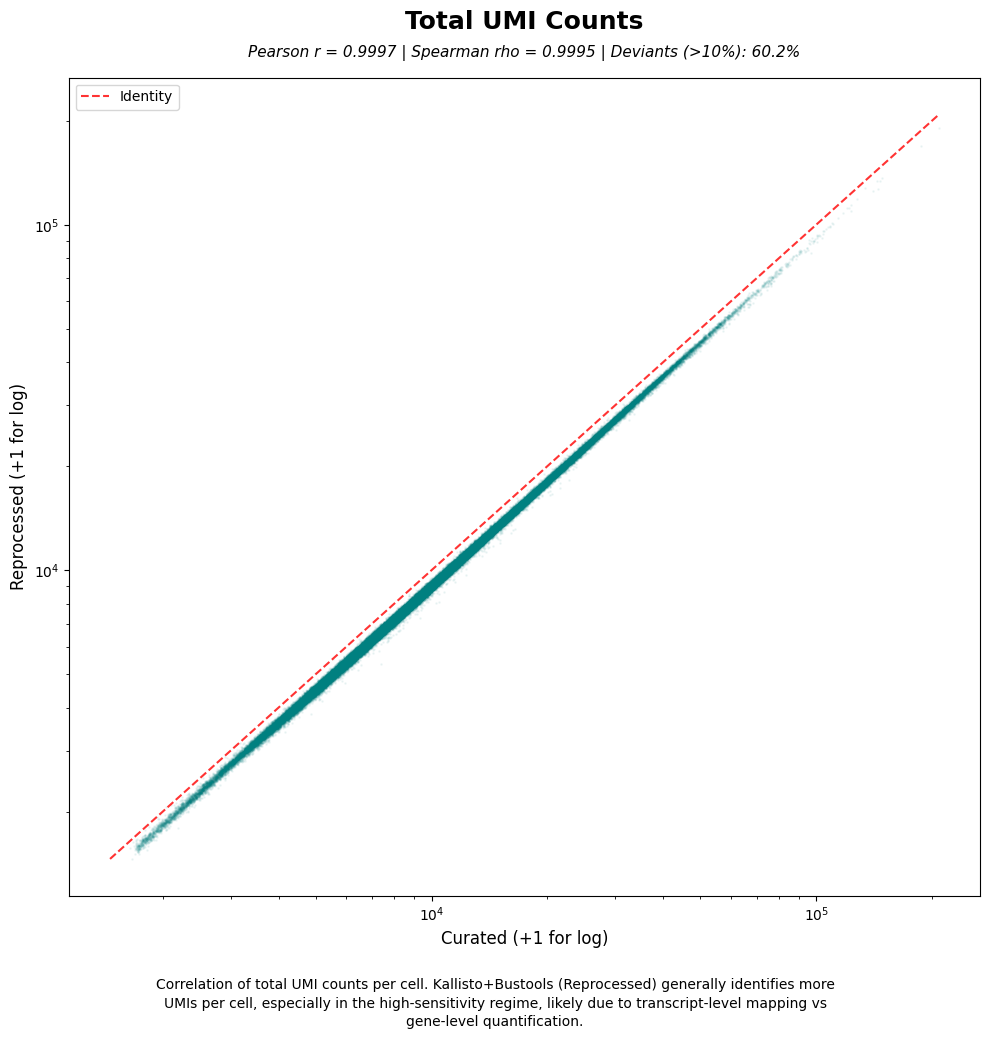
\includegraphics[width=\linewidth,height=0.78\textheight,keepaspectratio]{umi.png}
        \end{column}
        \begin{column}{0.49\textwidth}
            \centering
            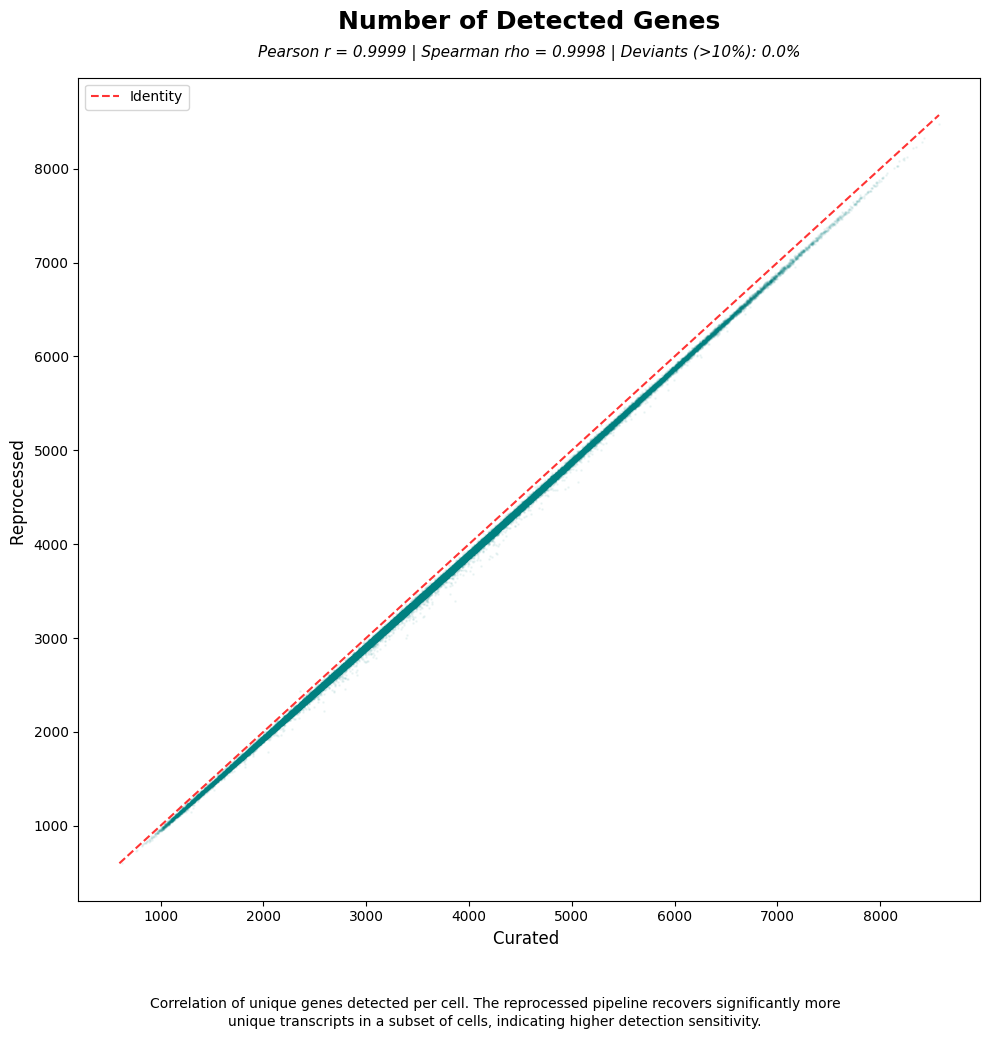
\includegraphics[width=\linewidth,height=0.78\textheight,keepaspectratio]{genes.png}
        \end{column}
    \end{columns}
\end{frame}

\begin{frame}{Gene-Level Expression Agreement}
    \begin{columns}[T,onlytextwidth]
        \begin{column}{0.49\textwidth}
            \centering
            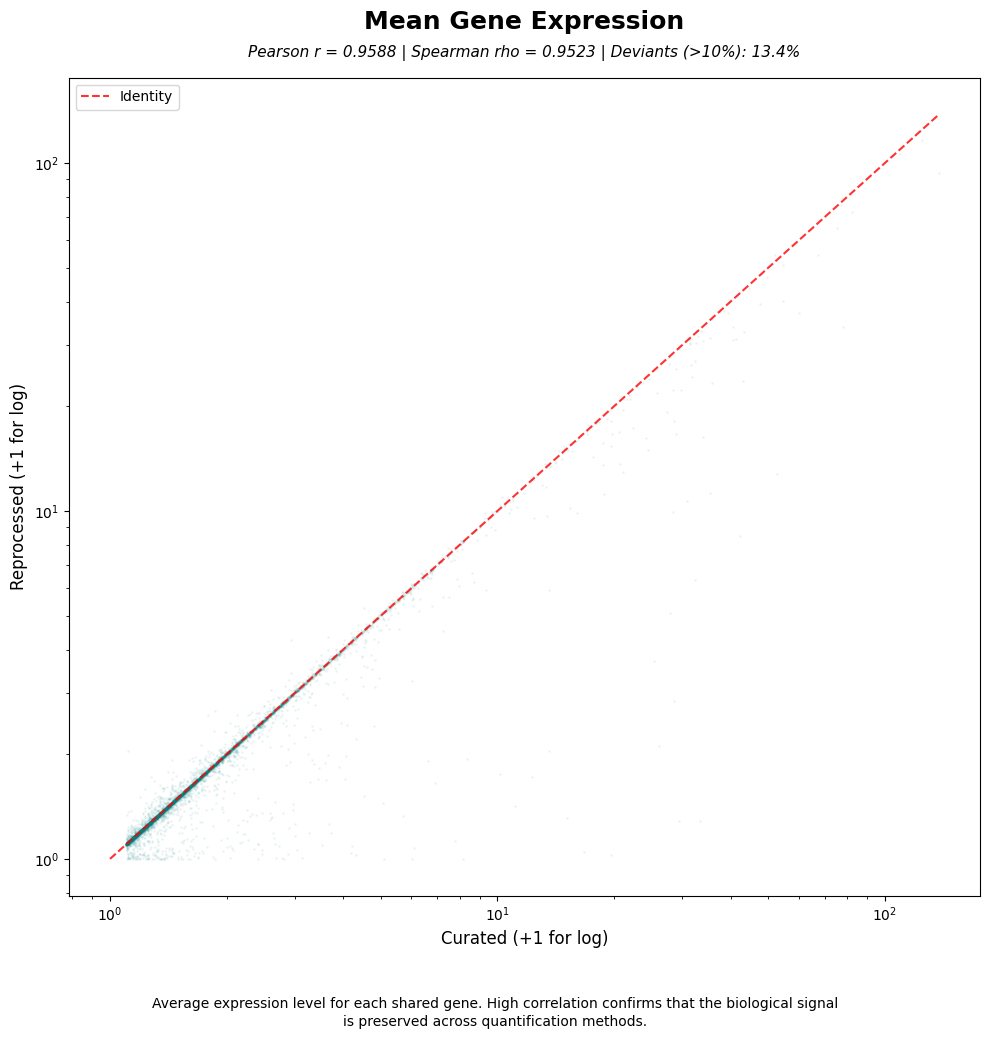
\includegraphics[width=\linewidth,height=0.78\textheight,keepaspectratio]{expression.png}
        \end{column}
        \begin{column}{0.49\textwidth}
            \centering
            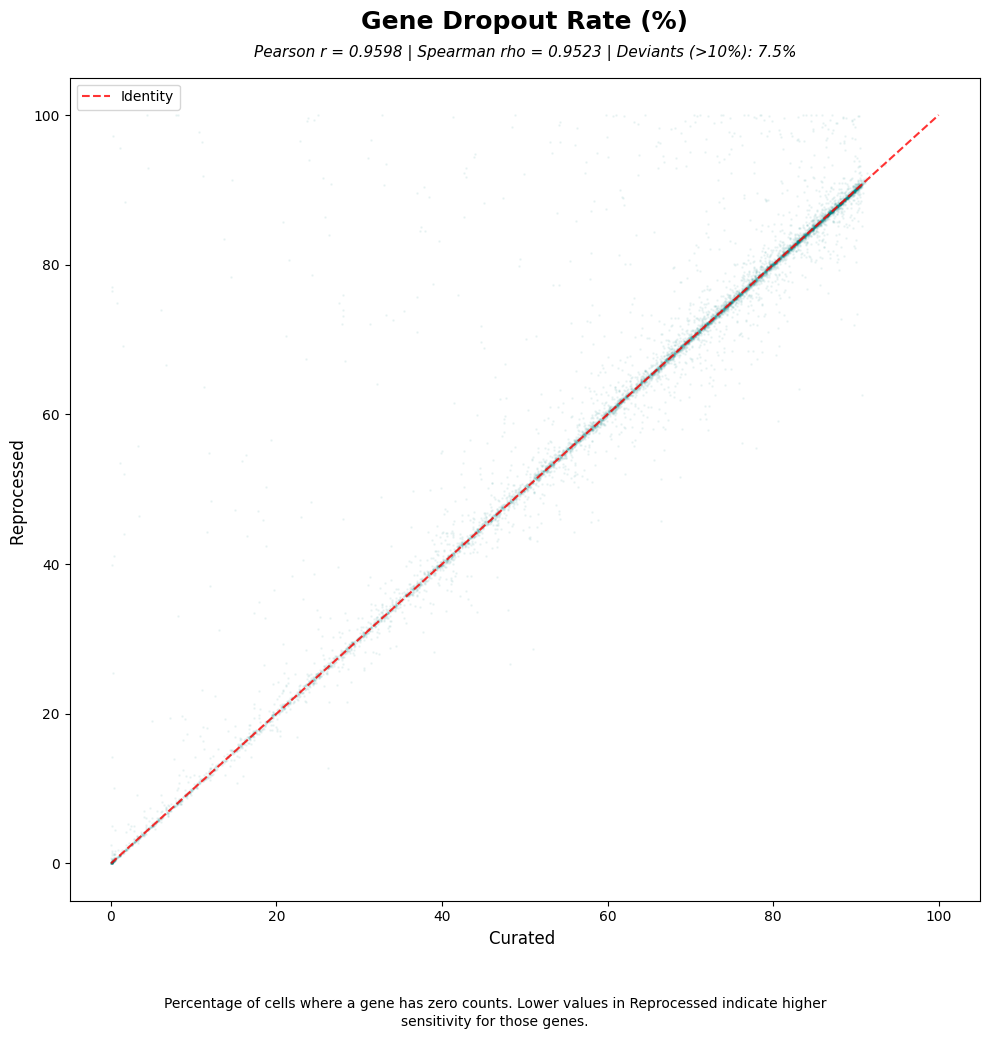
\includegraphics[width=\linewidth,height=0.78\textheight,keepaspectratio]{dropout.png}
        \end{column}
    \end{columns}
\end{frame}

\begin{frame}{Expression Vectors Are Preserved}
    \begin{itemize}
        \item For each shared cell, we compare the original and reprocessed expression vectors over the same genes.
        \item The histogram shows the distribution of Pearson correlation values for a sample of 10,000 cells.
    \end{itemize}
    \vspace{0.5em}
    \centering
    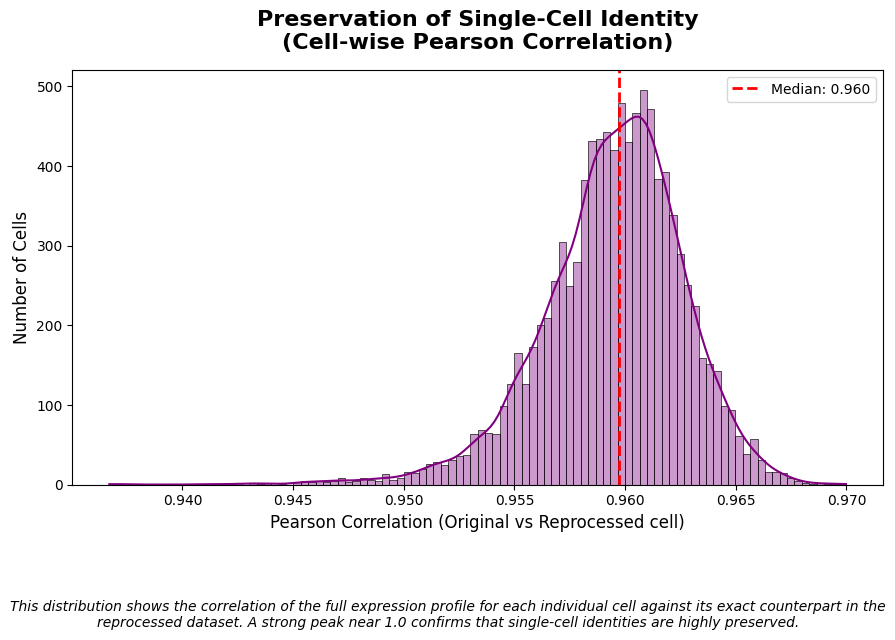
\includegraphics[width=0.7\linewidth,height=0.6\textheight,keepaspectratio]{pearson_per_cell.png}
\end{frame}

\begin{frame}{Guide Recovery: Mixture Model Approach}
    \begin{itemize}
        \item We use a \textbf{Gaussian-Poisson mixture model} to separate guide signal from background.
        \item The background is modeled as a Poisson distribution, while the true signal follows a Gaussian distribution.
        \item The decision threshold is automatically set at the crossover point where the probability of signal becomes higher than background.
        \item Cells are assigned a guide if at least one probe targets the gene and passes this threshold.
        \item Result: \textbf{205,457 / 214,522 (95.8\%)} of cells match the original study assignments.
    \end{itemize}
\end{frame}

\begin{frame}{What We Have Now}
    \begin{itemize}
        \item A working, reproducible FASTQ-to-H5AD pipeline for perturb-seq datasets.
        \item Both expression and guide calling are solved with very good alignment to original data.
        \item A comparison workflow that checks cell-level expression, gene-level expression, dropout, and perturbation labels.
        \item Pipeline is ready to scale to other datasets in the catalogue.
    \end{itemize}
\end{frame}

\begin{frame}{Next Steps}
    \begin{itemize}
        \item \textbf{Parameter fine-tuning:} Optimizing the mixture model components for better signal separation.
        \item \textbf{Scale-out:} Start running the pipeline for all other available perturb-seq datasets.
        \item \textbf{Downstream analysis:} Run distance metrics between genes, plus the existing DEA and GSEA workflows.
        \item \textbf{Feedback:} This meeting is the last opportunity for feedback before we begin full-scale processing.
    \end{itemize}
\end{frame}

\end{document}
